\documentclass[writeup.tex]{subfiles}
\begin{document}

\section{Part 2: Awesome Package Konveyance} \label{section.part2}
	Well, the task is clear, it's time to extract the APK from the zip file.\\
	\\
	... A minor roadblock, the ZIP file is password protected but a lucky guess that the password is "bugbounty" and the APK is extracted.\\
	\\
	Perfect, let us proceed.
	
	\subsection{What username and password are embedded in the APK file?}
		The right tool to answer this question seems to be jadx\footnote{The GitHub repository can be found at \url{https://github.com/skylot/jadx}.} this is also the tool suggested by one of the elves, Shinny Upatree.\\
		\\
		With the APK opened in jadx, there are a few options as to finding the embedded username and password. Option one, browse through the source code for the application, which can be found in the package "com.northpolewonderland.santagram", this can be seen in \autoref{fig.jadx_package_explorer}.
		
		\begin{figure}[H]
			\centering
			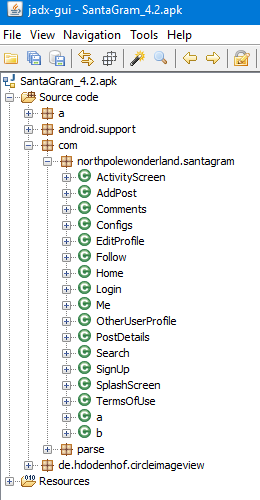
\includegraphics[scale=.7]{screenshots/jadx_package_explorer}
			\caption{jadx package explorer of SantaGram}
			\label{fig.jadx_package_explorer}
		\end{figure}
		
		Or, and personally I like this better, perhaps try and get lucky and use the search feature to search for "username". The results of this search can be seen in \autoref{fig.jadx_search} and shows that there indeed is a username present.
		
		\begin{figure}[H]
			\centering
			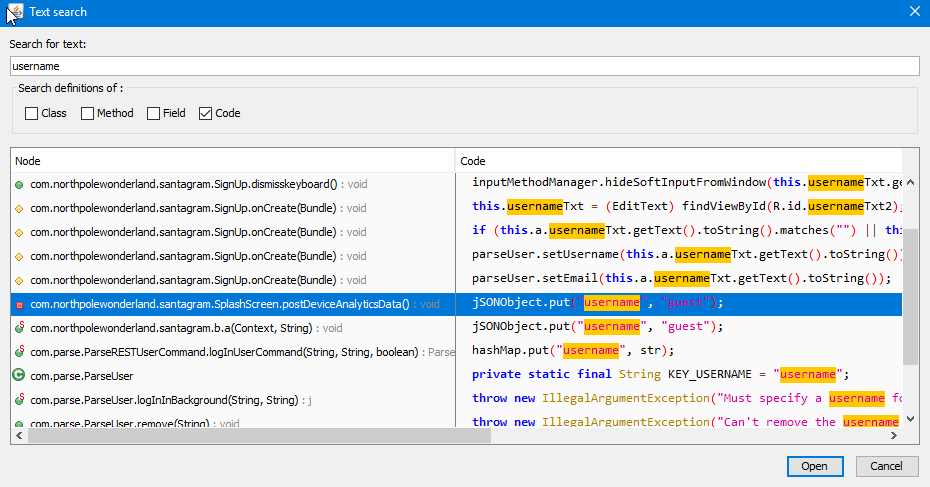
\includegraphics[width=\linewidth]{screenshots/jadx_search}
			\caption{jadx search results}
			\label{fig.jadx_search}
		\end{figure}
		
		Time to open the SplashScreen file to take a closer look, and you wouldn't have guessed it, but alongside that username,there is also a password. Check \autoref{fig.jadx_splashscreen} and have a look for yourself.

		\begin{figure}[H]
			\centering
			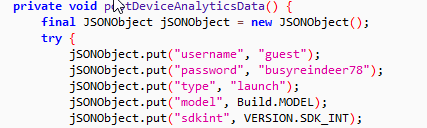
\includegraphics[scale=1]{screenshots/jadx_splashscreen}
			\caption{jadx SplashScreen}
			\label{fig.jadx_splashscreen}
		\end{figure}
		
		So there we have it, the embedded username and password.
		
	\subsection{What is the name of the audible component (audio file) in the SantaGram APK file?}
		Right, okay. So to get to the audio file inside the APK, let's unpack it, it's basically a ZIP file. Now this is another part were I happened to get very lucky. Check out \autoref{fig.unzip_santagram} to see why.

		\begin{figure}[H]
			\centering
			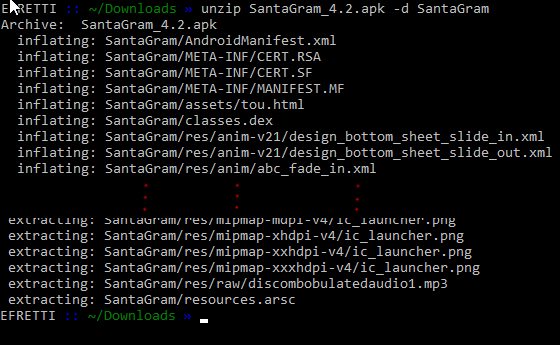
\includegraphics[scale=1]{images/unzip}
			\caption{Unzipping the SantaGram APK.}
			\label{fig.unzip_santagram}
		\end{figure}		
		
		As you can see, the second last line actually shows the file that we're looking for. To make sure, I did scroll through all of the output of the 'unzip' command.\\
		\\
		But there we have it folks, another challenge down.
		
\end{document}